\section{分布族的紧性}
\label{sec:weak-tightness}

前两节的判据都要先猜出极限分布，再去验证。很多时候极限并不知道，需要先判断一列分布有没有可能收敛到某个分布。实数列的情形可以作参照：有界数列不一定收敛，但总有收敛子列（Bolzano--Weierstrass定理）；无界数列可能连收敛子列都没有。分布列中扮演“无界”角色的，是概率质量逃向无穷远。

\paragraph{质量的逃逸}
$\delta_n$的全部质量跑到无穷远，分布函数对每个$x$都趋于$0$。逃逸也可以只是部分的。设$X_n\sim\mathcal{N}(0,n)$，则
\[
 F_n(x)=\Phi\bigl(x/\sqrt{n}\bigr)\longrightarrow\Phi(0)=\frac12,\qquad x\in\mathbb{R} .
\]
一半质量逃向$+\infty$，一半逃向$-\infty$，逐点极限是常数$1/2$，不是分布函数。再看$P_n=\frac12\delta_0+\frac12\delta_n$，它的分布函数趋于$\frac12\mathbf{1}_{\{x\geq0\}}$：留在原地的一半质量还在，跑远的一半消失了。图~\ref{fig:weak-mass-escape}画出这两种情形，它们都不可能弱收敛到任何概率分布。

\begin{BookInlineFigure}
 \centering
 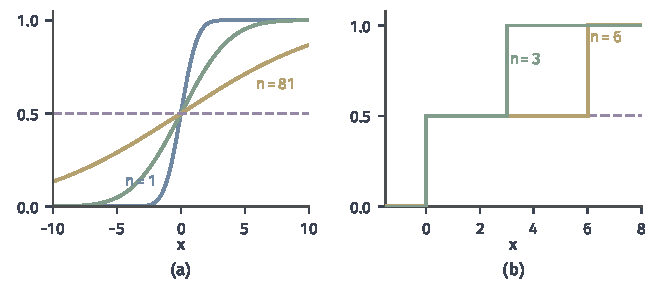
\includegraphics[width=112mm]{figures/07-probability/03-probability-limits/matplotlib/weak-mass-escape/figure.pdf}
 \caption{概率质量逃向无穷远。(a)$\mathcal{N}(0,n)$的分布函数，$n=1$（蓝）、$9$（绿）、$81$（黄），逐点趋于常数$1/2$（紫色虚线）。(b)$\frac12\delta_0+\frac12\delta_n$的分布函数，$n=3$（绿）与$n=6$（黄）；逐点极限$\frac12\mathbf{1}_{\{x\geq0\}}$（紫色虚线）的总质量只有$1/2$。}
 \label{fig:weak-mass-escape}
\end{BookInlineFigure}

\subsection{概率质量的控制}
\label{sec:weak-mass-control}

要防止逃逸，就要求所有分布在远处的质量能被同一个界控制。对单个分布这总能做到，因为$P(\lVert\bm{x}\rVert_2>r)$随$r\to\infty$趋于零；困难在于对一整族分布同时做到。

\begin{definition}[胎紧]
\label{def:weak-tight}
设$\{P_i\}_{i\in I}$是$\mathbb{R}^{d}$上的一族概率分布。若对每个$\varepsilon>0$，存在$r>0$使
\begin{equation}
 \sup_{i\in I}P_i\bigl(\{\bm{x}:\lVert\bm{x}\rVert_2>r\}\bigr)\leq\varepsilon ,
 \label{eq:weak-tight}
\end{equation}
则称这族分布\term{胎紧}（tight），也简称紧。一族随机向量称为胎紧，是指它们的分布胎紧。
\end{definition}

$\mathbb{R}^{d}$中有界闭集是紧集，所以式~\eqref{eq:weak-tight}也可以说成：存在紧集$K$，使每个$P_i$在$K$外的质量都不超过$\varepsilon$。单个分布胎紧；有限个胎紧族的并仍然胎紧，取各自的$r$中最大的一个即可。

直接验证式~\eqref{eq:weak-tight}往往不方便，矩的一致界给出常用的充分条件。

\begin{theorem}[矩的一致界蕴含胎紧]
\label{thm:weak-moment-tight}
设存在$p>0$与$M<\infty$，使$\mathbb{E}[\lVert\bm{X}_i\rVert_2^{p}]\leq M$对一切$i\in I$成立，则$\{\bm{X}_i\}_{i\in I}$胎紧，并且
\begin{equation}
 \sup_{i\in I}\mathbb{P}\bigl(\lVert\bm{X}_i\rVert_2>r\bigr)\leq\frac{M}{r^{p}},\qquad r>0 .
 \label{eq:weak-moment-tight}
\end{equation}
\end{theorem}

\begin{proof}
对非负变量$\lVert\bm{X}_i\rVert_2^{p}$用第~\ref{chap:tail-probabilities}章的Markov不等式，
\[
 \mathbb{P}\bigl(\lVert\bm{X}_i\rVert_2>r\bigr)\leq\mathbb{P}\bigl(\lVert\bm{X}_i\rVert_2^{p}\geq r^{p}\bigr)\leq\frac{M}{r^{p}} .
\]
取$r=(M/\varepsilon)^{1/p}$即得式~\eqref{eq:weak-tight}。
\end{proof}

对照前面的例子。$X_n\sim\operatorname{Bin}(n,2/n)$的期望恒为$2$，取$p=1$得$\mathbb{P}(X_n>r)\leq2/r$，胎紧。格点均匀分布都在$[0,1]$中，取$r=1$时式~\eqref{eq:weak-tight}左边为零。$\mathcal{N}(0,n)$的方差$n$没有一致界，它确实不胎紧：对任意固定的$r$，
\[
 \mathbb{P}(\lvert X_n\rvert>r)=2\bigl(1-\Phi(r/\sqrt{n})\bigr)\longrightarrow1 .
\]

\paragraph{胎紧与一致可积}
第~\ref{chap:random-variable-convergence}章的一致可积性也控制尾部，但控制的量不同。实随机变量族$\{X_i\}$一致可积，是指
\[
 \lim_{r\to\infty}\sup_{i\in I}\mathbb{E}\bigl[\lvert X_i\rvert\mathbf{1}_{\{\lvert X_i\rvert>r\}}\bigr]=0 .
\]
胎紧只数远处有多少质量；一致可积还要乘上质量所在的位置$\lvert x\rvert$，像力矩一样，远处的少量质量会被放大。在事件$\lvert X_i\rvert>r$上$\lvert X_i\rvert$至少是$r$，取期望得
\[
 \mathbb{P}\bigl(\lvert X_i\rvert>r\bigr)\leq\frac1r\,\mathbb{E}\bigl[\lvert X_i\rvert\mathbf{1}_{\{\lvert X_i\rvert>r\}}\bigr] ,
\]
所以一致可积蕴含胎紧。

反过来不成立。设$X_n$以概率$1/n$取$n$，以概率$1-1/n$取$0$。对$r\geq1$，只有$n>r$的那些$X_n$在$r$外有质量，质量为$1/n<1/r$，所以
\[
 \sup_{n}\mathbb{P}(X_n>r)\leq\frac1r,\qquad \sup_{n}\mathbb{E}\bigl[X_n\mathbf{1}_{\{X_n>r\}}\bigr]=\sup_{n>r}n\cdot\frac1n=1 .
\]
这族变量胎紧，却不一致可积。远处的质量$1/n$越来越少，而它与位置$n$的乘积始终是$1$。图~\ref{fig:weak-tight-vs-ui}对比了这两个量。第~\ref{sec:weak-integral-limits}节将看到，这个差别决定了期望能否随分布取极限。

\begin{BookInlineFigure}
 \centering
 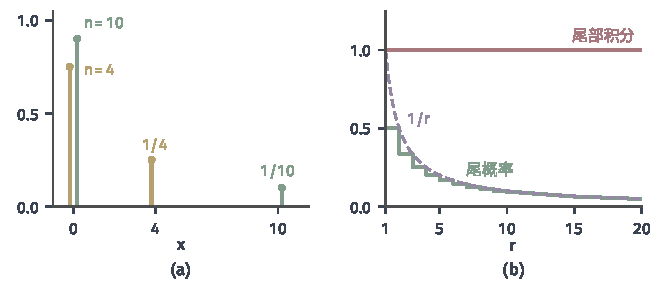
\includegraphics[width=112mm]{figures/07-probability/03-probability-limits/matplotlib/weak-tight-vs-ui/figure.pdf}
 \caption{胎紧与一致可积的差别，$X_n$以概率$1/n$取$n$，否则取$0$。(a)$n=4$（黄）与$n=10$（绿）的质量；远处质点很轻，乘以位置后都等于$1$。(b)作为$r$的函数，$\sup_n\mathbb{P}(X_n>r)$（绿）趋于零，紫色虚线为上界$1/r$；$\sup_n\mathbb{E}[X_n\mathbf{1}_{\{X_n>r\}}]$（红）恒为$1$。}
 \label{fig:weak-tight-vs-ui}
\end{BookInlineFigure}

\subsection{弱收敛子列}
\label{sec:weak-subsequences}

胎紧在分布列中的作用，正如有界性在实数列中的作用。下面的定理是Bolzano--Weierstrass定理的对应物。

\begin{theorem}[胎紧与弱收敛子列]
\label{thm:weak-prokhorov}
设$\{P_n\}$是$\mathbb{R}^{d}$上的概率分布列。
\begin{enumerate}
 \item 若$\{P_n\}$胎紧，则存在子列$P_{n_k}$与概率分布$P$，使$P_{n_k}\xrightarrow{\mathrm{w}}P$。
 \item 若一族分布中任取的序列都有弱收敛到概率分布的子列，则这族分布胎紧。
\end{enumerate}
\end{theorem}

后一条中的性质称为弱收敛意义下的相对紧。所以在$\mathbb{R}^{d}$中，胎紧与相对紧是同一回事。下面对$d=1$证明第一条，并对一般$d$证明第二条。

\begin{proof}
(1)，$d=1$。记$F_n$为$P_n$的分布函数，分四步。

第一步，用对角线方法在有理点上取收敛子列。把有理数排成$q_1,q_2,\dots$。数列$\bigl(F_n(q_1)\bigr)$在$[0,1]$中，有收敛子列；在这个子列中再取使$F_n(q_2)$收敛的子列，如此继续。取第$k$次所得子列的第$k$项，得到子列$(n_k)$，使对每个有理数$q$，$F_{n_k}(q)$收敛到某个$G(q)\in[0,1]$。$G$在有理数上不减。

第二步，构造右连续的极限。令
\[
 F(x)=\inf\{G(q):q\text{为有理数},\,q>x\} .
\]
$F$不减。若$x_m\downarrow x$，对每个有理数$q>x$，$m$足够大时$q>x_m$，于是$F(x_m)\leq G(q)$；对$q$取下确界得$\lim_mF(x_m)\leq F(x)$，而单调性给出反向不等式，所以$F$右连续。

第三步，在$F$的连续点$x$处证明$F_{n_k}(x)\to F(x)$。任取$\varepsilon>0$。由左连续性，取$y<x$使$F(y)>F(x)-\varepsilon$；由$F(x)$的定义，取有理数$s>x$使$G(s)<F(x)+\varepsilon$；再取有理数$r\in(y,x)$，由$F(y)$的定义有$F(y)\leq G(r)$。$F_{n_k}$不减，于是
\[
 \begin{aligned}
 \limsup_{k\to\infty}F_{n_k}(x)&\leq\lim_{k\to\infty}F_{n_k}(s)=G(s)<F(x)+\varepsilon,\\
 \liminf_{k\to\infty}F_{n_k}(x)&\geq\lim_{k\to\infty}F_{n_k}(r)=G(r)\geq F(y)>F(x)-\varepsilon .
 \end{aligned}
\]

第四步，用胎紧说明$F$是分布函数。对$\varepsilon>0$取式~\eqref{eq:weak-tight}中的$r$。对有理数$q>r$，$F_n(q)\geq1-\varepsilon$对一切$n$成立，所以$G(q)\geq1-\varepsilon$，从而$x\geq r$时$F(x)\geq1-\varepsilon$。对有理数$q<-r$，$F_n(q)\leq\varepsilon$，所以$x<q$时$F(x)\leq G(q)\leq\varepsilon$。因此$F(-\infty)=0$，$F(+\infty)=1$。不减、右连续且两端极限为$0$与$1$的函数是某个概率分布$P$的分布函数（第~\ref{chap:probability-spaces}章）。由定理~\ref{thm:weak-cdf-criterion}，$P_{n_k}\xrightarrow{\mathrm{w}}P$。

(2)，一般$d$。设这族分布不胎紧，则存在$\varepsilon>0$，对每个$m$都能在族中取到$P_m$，使$P_m(\lVert\bm{x}\rVert_2>m)>\varepsilon$。按假设，$(P_m)$有子列$P_{m_k}\xrightarrow{\mathrm{w}}P$。固定$r>0$，集合$\{\lVert\bm{x}\rVert_2\geq r\}$是闭集，当$m_k\geq r$时它包含$\{\lVert\bm{x}\rVert_2>m_k\}$。由Portmanteau定理的(3)，
\[
 P\bigl(\lVert\bm{x}\rVert_2\geq r\bigr)\geq\limsup_{k\to\infty}P_{m_k}\bigl(\lVert\bm{x}\rVert_2\geq r\bigr)\geq\varepsilon .
\]
这对每个$r$成立，与$P(\lVert\bm{x}\rVert_2\geq r)\to0$矛盾。
\end{proof}

第一步取出的极限$G$总存在，第四步之前的$F$也总能构造出来，胎紧只在第四步起作用。图~\ref{fig:weak-mass-escape}(b)就是缺了第四步的情形：前三步的构造给出$\frac12\mathbf{1}_{\{x\geq0\}}$，它右连续、不减，但$F(+\infty)=1/2$。$d>1$时第一条的证明思路相同，用多元分布函数在有理点上取对角线子列，细节较繁，可查阅~\scite{math-kallenberg2021probability}。

定理的第一条也称为\term{Helly选择定理}（Helly selection theorem）。在一般的完备可分度量空间上，胎紧（式~\eqref{eq:weak-tight}中的球换成紧集）与相对紧仍然等价，这就是\term{Prokhorov定理}（Prokhorov theorem）；空间的完备与可分保证单个分布胎紧，是相对紧推出胎紧所需的条件。本卷只在有限维空间中使用它。

\paragraph{子列极限的唯一性}
胎紧只保证有收敛子列，不保证整列收敛。$P_n$在$\delta_0$与$\delta_1$之间交替，所有质量都在$[0,1]$中，胎紧；偶数项与奇数项各自收敛，极限不同，整列不收敛。数列的情形也一样：有界数列收敛，当且仅当它所有收敛子列的极限相同。

\begin{lemma}[子列原则]
\label{lem:weak-subsequence}
设$\{P_n\}$胎紧，并且每个弱收敛的子列都收敛到同一个分布$P$，则$P_n\xrightarrow{\mathrm{w}}P$。
\end{lemma}

\begin{proof}
若不然，存在$f\in C_b(\mathbb{R}^{d})$、$\varepsilon>0$和子列$(n_k)$，使对一切$k$，
\[
 \Bigl\lvert\int f\,\mathrm{d}P_{n_k}-\int f\,\mathrm{d}P\Bigr\rvert\geq\varepsilon .
\]
子列仍胎紧，由定理~\ref{thm:weak-prokhorov}，它有进一步的子列弱收敛，按假设极限为$P$。沿这个进一步的子列，$\int f\,\mathrm{d}P_{n_k}\to\int f\,\mathrm{d}P$，与上式矛盾。
\end{proof}

这个引理把弱收敛的证明分成两件互相独立的事：用胎紧得到子列极限的存在，用别的办法证明子列极限只有一个。第~\ref{sec:weak-cf}节将用特征函数完成后一件事。
